%!TEX root = ../thesis.tex
%*******************************************************************************
%****************************** Fifth Chapter **********************************
%*******************************************************************************
\chapter{Ballistic Deposition on Square Lattice}
\label{chapter:ballistic-deposition}
% **************************** Define Graphics Path **************************
\ifpdf
    \graphicspath{{Chapter4/Figs/}{Chapter5/Figs/}{Chapter5/Figs/L0/}{Chapter5/Figs/L1/}{Chapter5/Figs/L2/}{Chapter5/Figs/traditional/}}
\else
    \graphicspath{{Chapter4/Figs/}{Chapter5/Figs/}{Chapter5/Figs/L0/}{Chapter5/Figs/L1/}{Chapter5/Figs/L2/}Chapter5/Figs/traditional/}
\fi


We investigate percolation by random sequential ballistic deposition (RSBD) on a square lattice with interaction range upto second nearest neighbors. The critical points $p_c$ and all the necessary critical exponents $\alpha$, $\beta$, $\gamma$, $\nu$ etc. are obtained numerically for  each range of interactions. Like  in its thermal counterpart, we find that the critical exponents of RSBD depend on the range of interactions and for a given range of interaction they obey the Rushbrooke inequality. Besides, we obtain the exponent $\tau$ which characterizes the cluster size distribution  function $n_s(p_c)\sim s^{-\tau}$ \ref{subsect:cluster-size-dist-func} and the fractal dimension $d_f$ that characterizes the spanning cluster at $p_c$ \ref{subsect:fractal-dim}. Our results suggest that the RSBD for each range of interaction belong to a new universality class which is in sharp contrast to earlier results of the only work that exhist on RSBD.
\\
Imagine a spherical shaped object, say marble, is thrown on top of a 2D square lattice structure. First possible scenario is that the marble will be deposited in the first encountered site in the lattice . Now if the first encountered site is not empty, the possible scenario is that the marble will go in any of the four direction, $+x$, $-x$, $+y$ or $-y$, assuming no other direction in between is allowed in the lattice.  Now if the first neighbor is not empty then the marble will continue to go on in the previously selected direction and choose the next neighbor. This is the main theme of this thesis.\\
In our experiment, we occupy a randomly chosen site if it is empty else we select one of its four neighbor to occupy if it is empty else select next neighbor in that direction and occupy that site if it is empty else ignore current iteration and choose another site randomly. This process is repeated until there is no empty site in the lattice. We call this process the ballistic deposition on the square lattice. We introduce 1st and 2nd nearest neighbor interaction in this way.



\section{Redefinition of Site Percolation}
	In site percolation we take a square lattice of length $L$ and we choose sites randomly and occupy them and measure cluster size with the number of site in a cluster. This is the traditional definition of site percolation.
	
	First let us discuss about two most important quantities of interests in the		theory of phase transition and critical phenomena are the		entropy $H$ and the order parameter $P$ since they are the		ones which define the order of transition. For instance,		in the first order transition there must be a jump or gap		in entropy at the critical point which is why first order 		transition requires latent heat. Similarly, the order parameter too must suffer a jump or discontinuity at the		critical point and that is the reason why in the first order transition new and old phase can coexist at the same		time. Besides, they are also used as a litmus test to		check whether the transition is accompanied by symmetry breaking or not. In the case of symmetry breaking,		the system undergoes a transition from the disordered		state, which is characterized by maximally high entropy,		to the ordered state, which is characterized by maximally		high order parameter. Such transition happens with an		abrupt or sudden change in $P$ and $H$ but without gap	or discontinuity at $p_c$.	
	\subsection{The problem with the old definition}
		If we use the traditional definition of site percolation we encounter some serious problem. Firstly, it violates the second law of thermodynamics which states entropy cannot decrease in a closed system \cite{Benguigui2013} which is discussed in section \ref{subsect:entropy-thermodynamics}. But the traditional definition gives a graph of entropy where entropy is zero at $p=0$ then entropy increases to a maximum value and again decreases to zero at $p=1$. Figure \ref{fig:entropy-traditional} show the graph of entropy using the traditional definition of site percolation. Although ignoring the part where $p \sim 0$ gives us the correct exponent from the derivative of entropy (specific heat) but it surely violates one of the fundamental laws of physics.
		\begin{figure}
			\captionsetup[subfigure]{width=0.9\textwidth}
			\begin{subfigure}{0.5\textwidth}
			\centering
			\includegraphics[width=7cm]{{{sq_lattice_site_percolation_periodic__entropy_by_site_-entropy}}}
			\caption{Entropy from the traditional definition of site percolation}
			\label{fig:entropy-traditional}				
			\end{subfigure}
			\begin{subfigure}{0.5\textwidth}
			\centering
			\includegraphics[width=7cm]{{{sq_lattice_site_percolation_periodic__entropy_by_site-entropy-order_parameter-traditional2-L400}}}
			\caption{Entropy from the traditional definition of site percolation}
			\label{fig:order-disorder-transition}
			\end{subfigure}
			\caption{Effect of traditional definition of site percolation}
		\end{figure}
		
		Secondly, it give raise to ambiguity at $p=0$. 		 We know phase transition is an order-disorder transition and system goes from ordered state to disordered state or vice versa. Therefore a system cannot be in both ordered state and disordered state at the same time. But the traditional definition of site percolation does not agree with this. We can see this in figure \ref{fig:order-disorder-transition} where normalized entropy and order parameter is plotted together. We can see that at $p=0$entropy, which represents disorder, is minimum  and order parameter, which represents order, is also zero. Thus the system is in both ordered and disordered state at  the same time. Which is a serious problem with the traditional definition of site percolation.
		
	\subsection{Solution to the problem}
		Our problem will be resolved if the entropy is maximum at $p=0$ and gradually decrease to minimum and order parameter is minimum at $p=0$ and gradually increase to maximum. Since bond percolation does not raise this problem, a closer look at it and comparing it with site percolation is the first thing to do.
		\subsubsection{Bond Percolation}
		 In bond percolation we occupy bond and measure occupation probability by the fraction of the occupied bond with respect to total number of bonds. And we measure cluster size with the number of sites in it. Here, in the initial state, there is no bond present but all the sites are. We simply occupy bonds to connect sites to form clusters. Thus initially all the clusters are of size $1$ (contains exactly one site) giving maximum entropy and minimum order parameter. 
		
		 The algorithm for bond percolation is as follows,
		 \begin{enumerate}
		 	\item take a square lattice of length $L$.
		 	\item fill all $L^2$ the sites initially.
		 	\item occupy a randomly chosen bond and it will join some clusters.
		 	\item each time a bond is occupied, it will get connected to two neighboring sites and will form a cluster of size $2$. Here cluster size by number of sites in it.
		 	\item if a bond is occupied and right next to it there is another occupied bond and they are connected by a site and a cluster of size $3$ will be formed.
		 	\item this process is repeated until all the bonds are occupied and only one cluster remains
		 \end{enumerate}
		 The formation of cluster is visualized in the figure \ref{fig:cluster_growth_bond_percolation}.
		 \begin{figure}
		 	\begin{subfigure}{.5\textwidth}
		 		\centering
		 		\includegraphics[width=.8\linewidth]{{{sq_lattice_bond_percolation_1_0}}}
		 		\caption{Initial state}
		 	\end{subfigure}
		 	\begin{subfigure}{.5\textwidth}
		 		\centering
		 		\includegraphics[width=.8\linewidth]{{{sq_lattice_bond_percolation_1_1}}}
		 		\caption{Iteraion 1}
		 	\end{subfigure}
		 	\begin{subfigure}{.5\textwidth}
		 		\centering
		 		\includegraphics[width=.8\linewidth]{{{sq_lattice_bond_percolation_1_2}}}
		 		\caption{Iteraion 2}
		 	\end{subfigure}
		 	\begin{subfigure}{.5\textwidth}
		 		\centering
		 		\includegraphics[width=.8\linewidth]{{{sq_lattice_bond_percolation_1_3}}}
		 		\caption{Iteraion 3}
		 	\end{subfigure}
		 	\caption{Growth of a Cluster in Bond Percolation on square Lattice}
		 	\label{fig:cluster_growth_bond_percolation}
		 \end{figure}
		
		
		Keeping this in mind one might guess the possible rule for site percolation. We should have a lattice of $2 L^2$ bonds and no sites and we should occupy site and connect bonds with sites to form clusters. As usual the occupation probability will be measured by $n/L^2$ where $n$ is the number of occupied sites. In this way we have maximum entropy and minimum order parameter at $p=0$ see figure \ref{fig:ordered-disordered-transition}.
		
		\subsubsection{Site Percolation}
		The algorithm for site percolation is as follows,
		\begin{enumerate}
			\item take a square lattice of length $L$.
			\item fill all $2 L^2$ bonds initially.
			\item occupy a randomly chosen site and it will join some clusters.
			\item each time a site is occupied, it will get connected to four neighboring bonds and will form a cluster of size $4$. Note that we define cluster size by number of bonds in it.
			\item if a site is occupied and right next to it there is another occupied site and a cluster of size $7$ will be formed.
			\item this process is repeated until all the sites are occupied and only one cluster remains
		\end{enumerate}
		The formation of cluster is visualized in the figure \ref{fig:cluster_growth_site_percolation}.
		
		\begin{figure}
			\begin{subfigure}{.5\textwidth}
				\centering
				\includegraphics[width=.8\linewidth]{{{sq_lattice_site_percolation_1_0}}}
				\caption{Initial state}
			\end{subfigure}
			\begin{subfigure}{.5\textwidth}
				\centering
				\includegraphics[width=.8\linewidth]{{{sq_lattice_site_percolation_1_1}}}
				\caption{Iteraion 1}
			\end{subfigure}
			\begin{subfigure}{.5\textwidth}
				\centering
				\includegraphics[width=.8\linewidth]{{{sq_lattice_site_percolation_1_2}}}
				\caption{Iteraion 2}
			\end{subfigure}
			\begin{subfigure}{.5\textwidth}
				\centering
				\includegraphics[width=.8\linewidth]{{{sq_lattice_site_percolation_1_3}}}
				\caption{Iteraion 3}
			\end{subfigure}
			
			\caption{Growth of a Cluster in Site Percolation on square Lattice}
			\label{fig:cluster_growth_site_percolation}
		\end{figure}
	
	
	
		 Thus we can give the definition of site(bond) percolation. Take a square lattice of length $L$ with $L^2$ sites and $2L^2$ bonds. In site(bond) percolation all the bonds(sites) are present initially and occupy sites(bonds) to connect bonds(sites) in order to form cluster. Measure occupation probability as a fraction of sites(bonds) with respect to total sites(bonds) \cite{redefinition-of-site-percolation}.
		 
	\subsection{Impact of the new definition}
		The new definition resolves the problems of the traditional definition of site percolation. It does not violet the second law of thermodynamics. Which means that initially at $p=0$ the entropy is maximum and the order parameter is minimum. As we occupy sites and form clusters the entropy decreases. At the critical point the rate of decreasing entropy is maximum. At $p=1$, when all the sites are occupied, there exists only one cluster giving minimum entropy and maximum order parameter \ref{fig:entropy}.		Thus ambiguity of being in ordered and disordered state at the same time is resolved \ref{fig:order-disorder-transition}. Also the critical exponents are unchanged by the new definition. Thus site and bond percolation belong to a universality class \cite{Hassan2015, Hassan2016}.


\section{Structure and Algorithm}
Random percolation (RP) model can also be seen as a random sequential adsorption (RSA) process of particles on a given substrate to form monolayers of clusters of complex shape and structures. In RSA, a site is first picked at random and it is occupied if it is empty and the trial attempt is rejected if it is already occupied. We shall first show that this process too reproduce all the existing results of the CRP including the $p_c$ value. We can modify the rejection criterion. First, we assume that the adsorbing particles are hard sphere and impenetrable. Then we assume that if a particle fall onto an already adsorbed particle it is not straightaway rejected. Instead, it is allowed to roll down over the already deposited particle to one of its nearest neighbours at random following the steepest descent path. The particle is then adsorbed permanently if the nearest neighbour is empty else the trial attempt is rejected. This is known as the ballistic deposition (BD) model for $l = 1$. We also consider the case that if the nearest neighbour is occupied then the incoming particle attempt to push the neighbour to its next neighour site along the same line to make room for itself. However, the trial attempt of pushing the neighbour is successful if the next neibhouring site along the same line is empty else the trial attempt is discarded. We regard it as BD model for $l = 2$ while the classical percolation correspond to BD model with $l = 0$. Our primery goal is to prove that the critical exponents of percolation changes as changes as we increase the range of interaction like we find in its thermal counterpart. We numerically find the various necessary critical exponents and find that BD for each different range of interaction belong to different universality class and each universality class
obeys the Rusbrooke inequality.\\

Percolation is all about configuration of clusters of deposited particles and the investigation of the emergence of a large-scale connected path created by clusters formed by contiguous diposoted particles. We use extensive Monte Carlo simulation on a square lattice with the usual periodic boundary condition to study site percolation according to RSBD rule.\\

The algorithm of the percolation by RSBD can be described as follows. We first label all the sites
row by row from left to right starting from the top left corner. That is, we first label the first row from
left to right as $i=1,2,...,L$, the second row again from left to right as $i=L+1,L+2,....,2L$
and we continue this till we reach the bottom row which we label as $i=(L-1)L+1,...,L^2$. 
Then at each step we pick a discrete random number $R$ from $1,2,...,L^2-1,L^2$ using uniform random number
generator and check if the site it represents is already occupied or not. If it is
empty we occupy it straightaway and move on to the next step. Else we pick one of its neighbours at random. 
The second attempt in the same step, that mimic the roll over mechanism, is successul if the neighbour
it picks is empty and if not the trial attempt to deposit is rejected permanently and we move on to the next 
step anyway. This process is
repeated over and over again till we want it to stop. We call it RSBD of degree one. We also consider
the case of RSBS of degree two where the trial attempt is made to occupy the second nearest neighbour too.
In this case if the incoming particle that fall onto an already occupied site and find its 
neighbour is ocupied too but the next nearest neighbour site is empty then the neighbour move to the empty
site to make space for the incoming perticle to be deposited there. 
\begin{enumerate}
	\item take a square lattice of length $L$.
	\item choose a site randomly
	\item if the chosen site is empty then occupy it else choose one of the four neighbor randomly
	\item if the chosen neighbor is empty then occupy it else choose second nearest neighbor in that direction
	\item if the second nearest neighbor is empty then occupy the site else ignore this step
\end{enumerate}


\section{Finding Numerical Values} 
\label{sect:finding-numerical-values}
	\subsection{Critical occupation probability, $p_c$} 
	\label{subsect:finding-pc}
	When we occupy sites of the square lattice, initially, there are only cluster of size $1$. As we keep occupying different size of clusters starts to appear. At a certain point a special cluster appears which spans the entire lattice. We call this cluster the \textit{Spanning Cluster}. It should be noted that the spanning cluster is a special property of the lattice and the appearance of the spanning cluster is the result of phase transition. At the point where the spanning cluster first appears is called the critical point and denoted by $p_c$, meaning the occupation probability at the critical point. The figure \ref{fig:spanning-probability} shows the graph of the spanning probability, $w(p,L)$, versus the occupation probability $p$ for different interactions ($L0, L1, L2$) for different lengths. We have found that $p_c$ is $0.5927, 0.5782, 0.5701$ for $L0, L1, L2$ respectively.Thus for long range interaction $p_c$ is smaller than for short range interaction. 
		\begin{figure}
			\begin{subfigure}{0.329\textwidth}
				\centering
				\includegraphics[width=\linewidth]{{{sq_lattice_site_percolation_periodic_-occupation_probability-pc0.5927}}}
				\caption{L0}
			\end{subfigure}
			\begin{subfigure}{0.329\textwidth}
				\centering
				\includegraphics[width=\linewidth]{{{sq_lattice_site_percolation_ballistic_deposition_L1_periodic_-occupation_probability-pc0.5782}}}
				\caption{L1}
			\end{subfigure}
			\begin{subfigure}{0.329\textwidth}
				\centering
				\includegraphics[width=\linewidth]{{{sq_lattice_site_percolation_ballistic_deposition_L2_periodic_-occupation_probability-pc0.5701}}}
			\caption{L2}
			\end{subfigure}
			\caption{Spanning Probability, $w(p,L)$ vs Occupation Probability, $p$}
			\label{fig:spanning-probability}
		\end{figure}
	The quantity $w(p, L)$ is called the spanning probability in a non periodic case and wrapping probability in a periodic case.
	The question is how do we find the wrapping probability, given that we have a list of $p_c$ for different length. Note that for a certain length $L$, in each realization the $p_c$ is not exact value, instead it is a range of values that contains the $p_c$. For example, say we have a lattice of length $200$ and for that we will have different $p_c$ at each realization. After an infinite number of experimentation we will have to take an average and that will give the exact value of $p_c$. But since it is practically impossible, we can find $p_{c_{avg}}$ for different lattice size then from the graph we can extrapolate the exact value of $p_c$ for infinite lattice. Here $p_{c_{avg}}$ is calculated from a finite set of $p_c$ for a certain length. This process is not good enough. Since it requires  $p_{c_{avg}}$'s for a number of lattice size which is very costly to obtain. But from the data, list of $p_c$'s for different length, we can find the cumulative frequency distribution. It is astonishing  that for all length the wrapping probability coincide at a specific point. This implies that if we could have an infinite system, the wrapping probability for that system would have gone through this same point. This means we got our critical point, $p_c$, as the intersection of the $w(p,L)$ for different lengths.
	\subsection{Spanning Probability and finding $1/\nu$} \label{subsect:spanning-probability-and-one-by-nu}
	From the figure \ref{fig:spanning-probability} we can see that, as we increase the length of the lattice the wrapping probability $w(p,L)$ moves closer and closer to the critical point. And if we draw a horizontal line at a certain height, say $y=0.1$, and find the intersection of this line with $w(p,L)$ for each length  and note the $p$ and if we plot $\log(L)$ vs $\log(p-p_c)$ we get the slope $1/\nu$. If we now use the finite size scaling (FSS) hypothesis
	\begin{equation}
		w = (p-p_c) L^{1/\nu}
	\end{equation}
	we get a very good data collapse for $L0,L1,L2$ and got $1/\nu$ as $0.75, 0.736, 0.721$ respectively which is shown in figure \ref{spanning-probability-data-collapse}. That is they are self-similar \ref{label}.
		\begin{figure}
			\begin{subfigure}{0.329\textwidth}
				\centering
				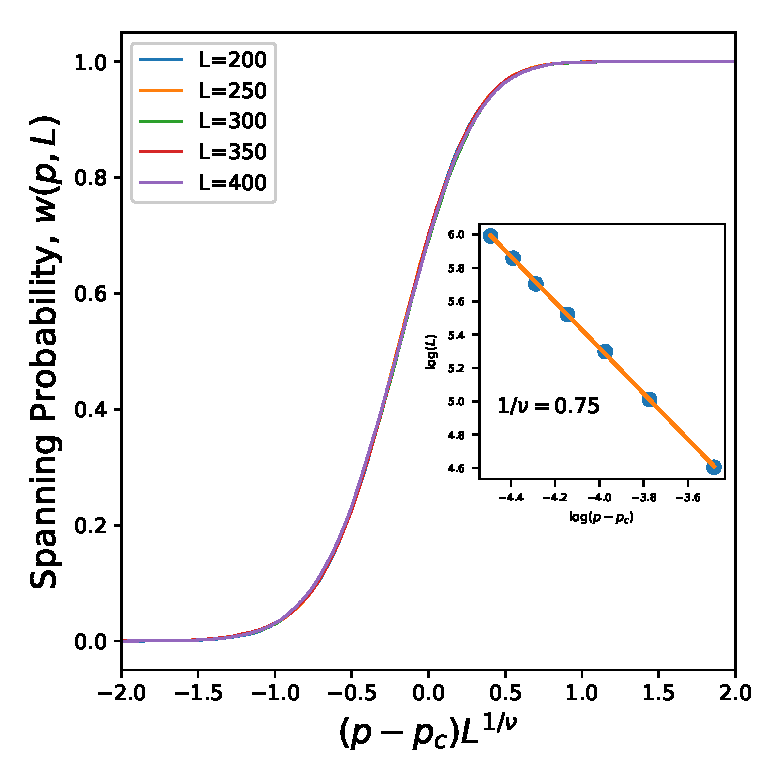
\includegraphics[width=\linewidth]{{{L0/sq_lattice_site_percolation_periodic_-occupation_probability-data_collapse-pc0.5927-ex0.7500}}}
				\caption{L0}
			\end{subfigure}
			\begin{subfigure}{0.329\textwidth}
				\centering
				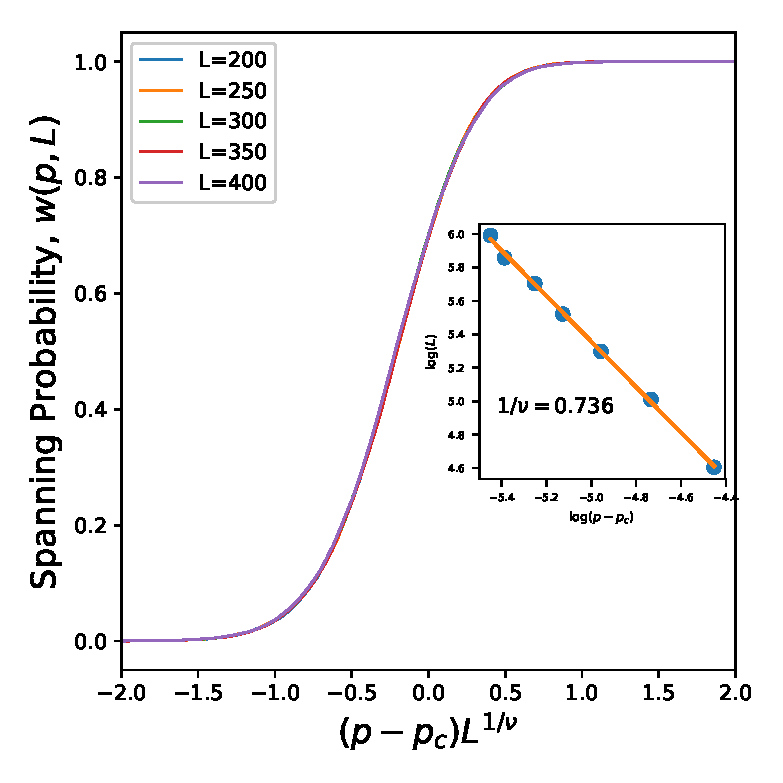
\includegraphics[width=\linewidth]{{{L1/sq_lattice_site_percolation_ballistic_deposition_L1_periodic_-occupation_probability-data_collapse-pc0.5782-ex0.7360}}}
				\caption{L1}
			\end{subfigure}
			\begin{subfigure}{0.329\textwidth}
				\centering
				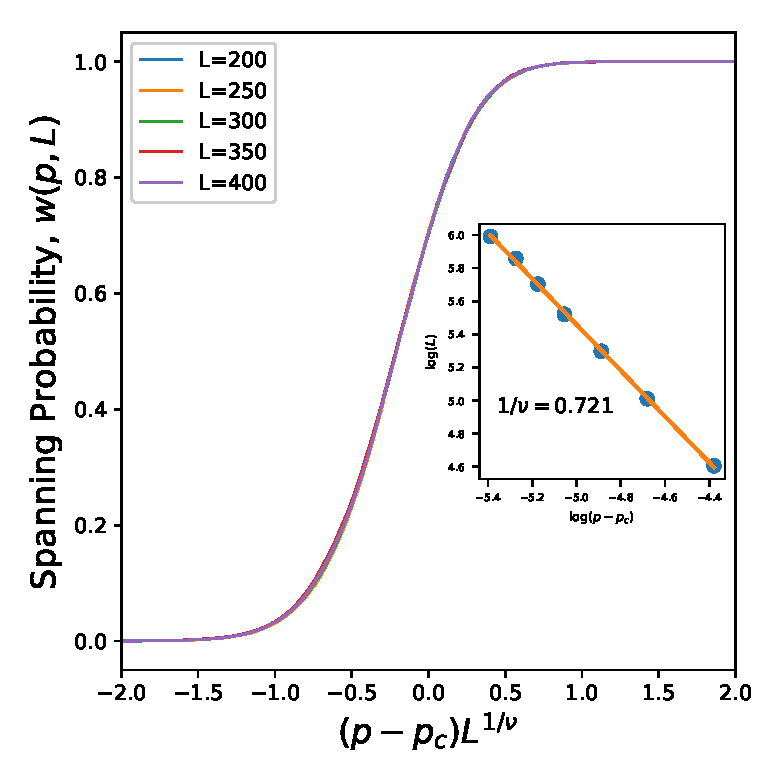
\includegraphics[width=\linewidth]{{{L2/sq_lattice_site_percolation_ballistic_deposition_L2_periodic_-occupation_probability-data_collapse-pc0.5701-ex0.7210}}}
				\caption{L2}
			\end{subfigure}
			\caption{$w(p,L)$ vs $(p-p_c) L^{1/\nu}$}
			\label{spanning-probability-data-collapse}
		\end{figure}
	
	\subsection{Entropy, Specific Heat and finding $\alpha$}
	\label{subsect:entropy-specific-heat}
		For any phase transition model the entropy is crucial. In percolation theory we use Shannon Entropy \cite{Shannon1948}. Using the definition \ref{label} we get the figure \ref{fig:entropy}
		\begin{figure}
			\begin{subfigure}{0.329\textwidth}
				\centering
				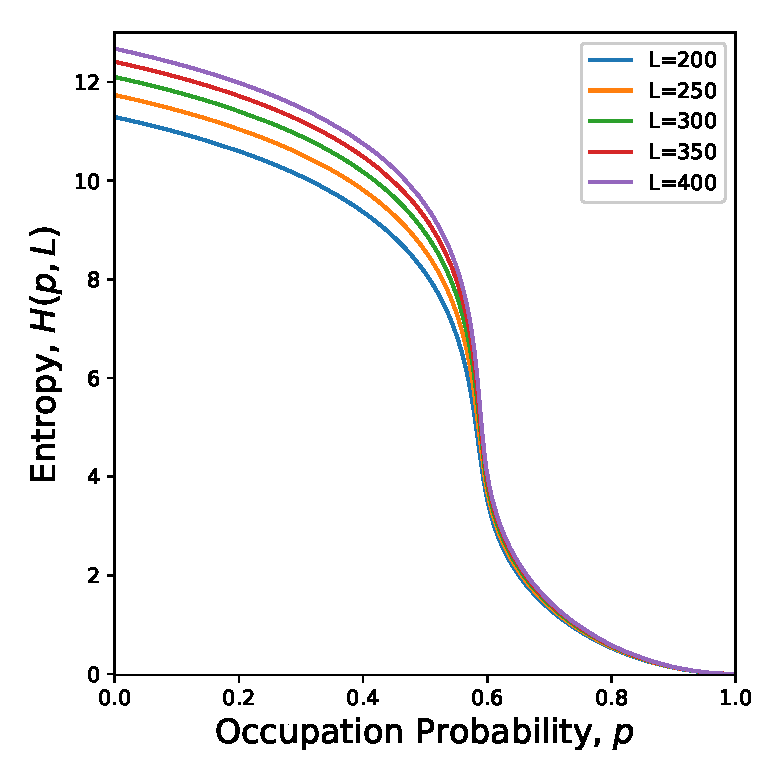
\includegraphics[width=\linewidth]{{{L0/sq_lattice_site_percolation_periodic_-entropy}}}
				\caption{L0}
			\end{subfigure}
			\begin{subfigure}{0.329\textwidth}
				\centering
				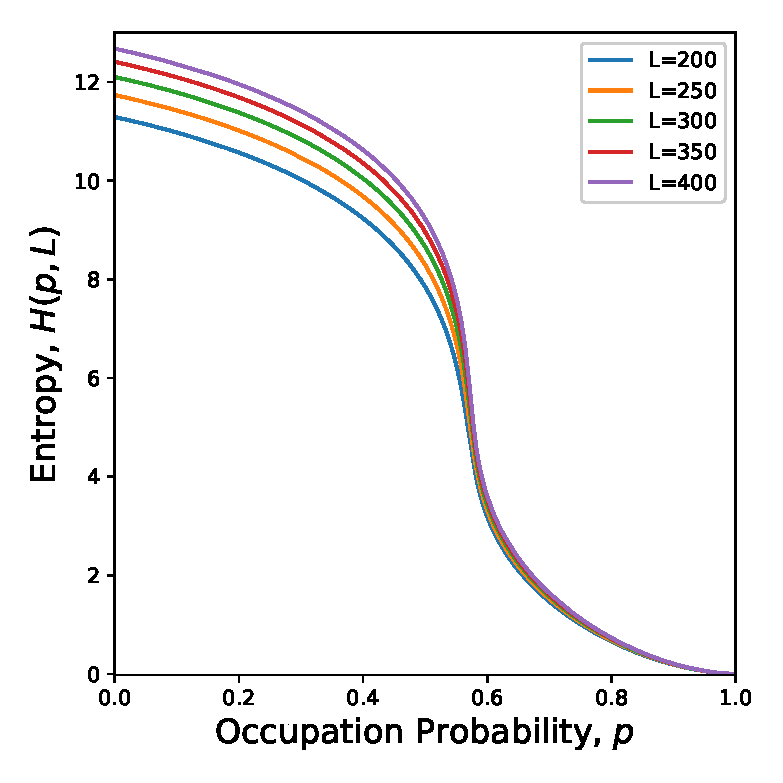
\includegraphics[width=\linewidth]{{{L1/sq_lattice_site_percolation_ballistic_deposition_L1_periodic_-entropy}}}
				\caption{L1}
			\end{subfigure}
			\begin{subfigure}{0.329\textwidth}
				\centering
				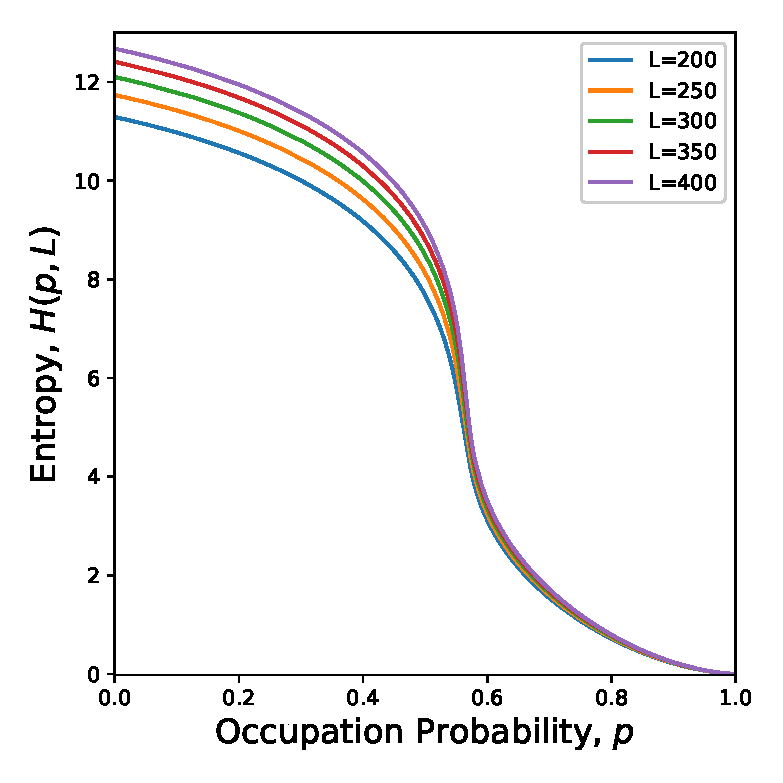
\includegraphics[width=\linewidth]{{{L2/sq_lattice_site_percolation_ballistic_deposition_L2_periodic_-entropy}}}
				\caption{L2}
			\end{subfigure}
			\caption{Entropy, $H(p,L)$ vs Occupation Probability, $p$}
			\label{fig:entropy}
		\end{figure}
	And since the specific heat $C(p,L)$ is nothing but the derivative of entropy, by simply differentiating entropy we get the specific heat (although we need to perform convolution\ref{} in order to get a smooth curve) shown in figure \ref{fig:specific-heat-graph}.
		\begin{figure}
			\begin{subfigure}{0.329\textwidth}
				\centering
				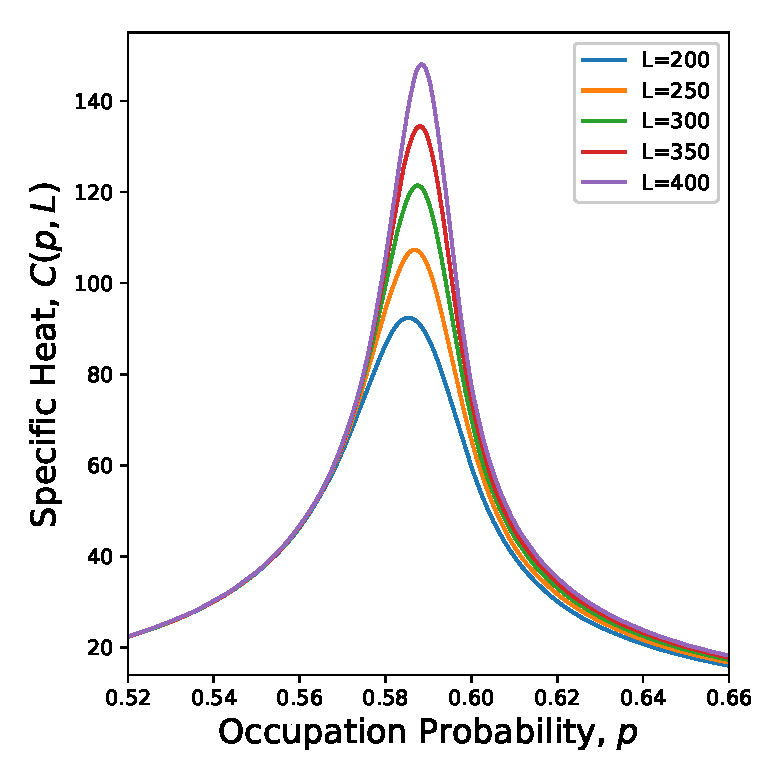
\includegraphics[width=\linewidth]{{{L0/sq_lattice_site_percolation_periodic__specific_heat-pc0.5927}}}
				\caption{L0}
			\end{subfigure}
			\begin{subfigure}{0.329\textwidth}
				\centering
				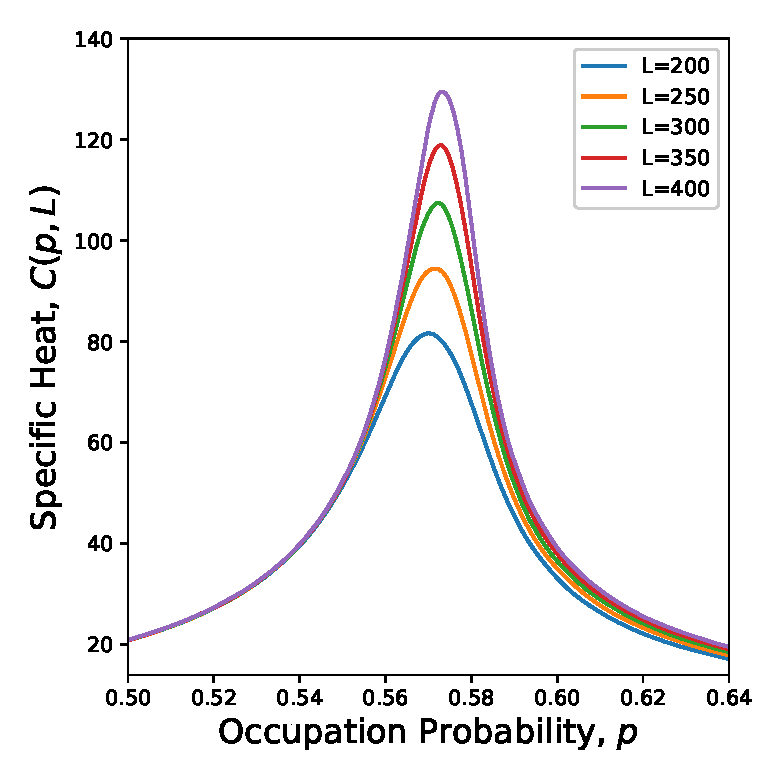
\includegraphics[width=\linewidth]{{{L1/sq_lattice_site_percolation_ballistic_deposition_L1_periodic__specific_heat-pc0.5782}}}
				\caption{L1}
			\end{subfigure}
			\begin{subfigure}{0.329\textwidth}
				\centering
				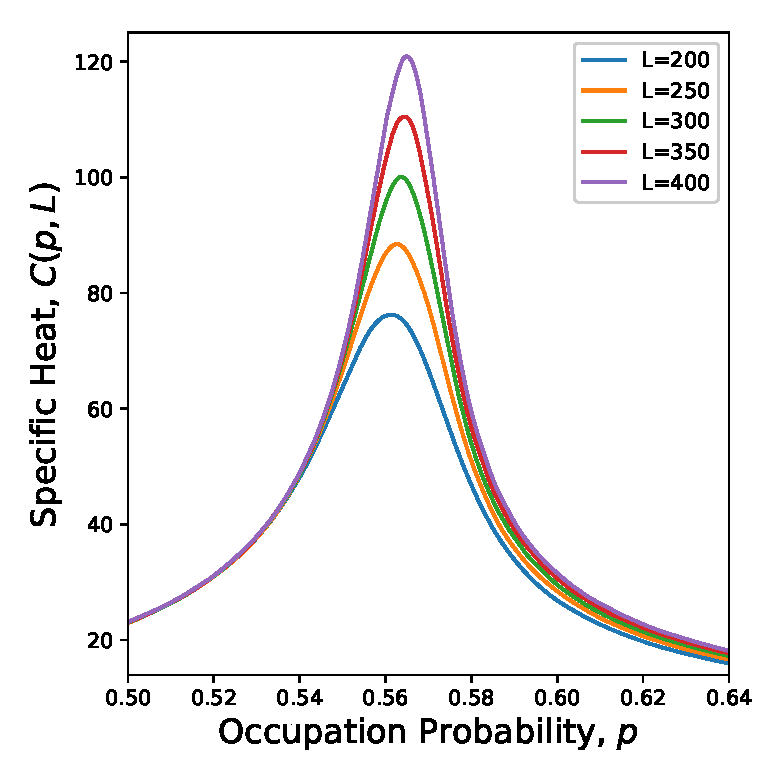
\includegraphics[width=\linewidth]{{{L2/sq_lattice_site_percolation_ballistic_deposition_L2_periodic__specific_heat-pc0.5701}}}
				\caption{L2}
			\end{subfigure}
			\caption{Specific Heat, $C(p,L)$ vs Occupation Probability, $p$}
			\label{fig:specific-heat-graph}
		\end{figure}
		From specific heat we can find the exponent $\alpha$. To do this first we need to scale the $x$-values of the specific heat data using the exponent $1/\nu$ obtained from \ref{subsect:spanning-probability-and-one-by-nu} and get the graph as in figure \ref{fig:specific-heat-x-scaled-graph}. From this graph we will not the height of each line and call it $C_h$. Since each line corresponds to a specific length $L$ we can plot $\log(C_h)$ versus $\log(L)$ and the absolute value of the graph will give $\alpha/\nu$ and from that we can find the exponent $\alpha$ simply by dividing $\alpha/\nu$ by $1/\nu$. We get $\alpha$ values $0.906,0.911,0.919$ for $L0,L1,L2$ correspondingly. and using this value we can apply FSS hypothesis to get data collapse.
		\begin{figure}
			\begin{subfigure}{0.329\textwidth}
				\centering
				\includegraphics[width=\linewidth]{{{sq_lattice_site_percolation_periodic__specific_heat-x-scaled-pc0.5927_alpha_0.6799_nu_0.750}}}
				\caption{L0}
			\end{subfigure}
			\begin{subfigure}{0.329\textwidth}
				\centering
				\includegraphics[width=\linewidth]{{{sq_lattice_site_percolation_ballistic_deposition_L1_periodic__specific_heat-x-scaled-pc0.5782_alpha_0.6712_nu_0.736}}}
				\caption{L1}
			\end{subfigure}
			\begin{subfigure}{0.329\textwidth}
				\centering
				\includegraphics[width=\linewidth]{{{sq_lattice_site_percolation_ballistic_deposition_L2_periodic__specific_heat-x-scaled-pc0.5701_alpha_0.6631_nu_0.721}}}
				\caption{L2}
			\end{subfigure}
			\label{fig:specific-heat-x-scaled-graph}
			\caption{$C(p,L)$ vs $(p-p_c) L^{1/\nu}$}
		\end{figure}
	If we plot $C L^{-\alpha/\nu}$ vs $(p-p_c)L^{1/\nu}$ we get perfect data collapse for $L0,L1,L2$ and it is shown in figure \ref{fig:specific-heat-data-collapse-graph}
		\begin{figure}
			\begin{subfigure}{0.329\textwidth}
				\centering
				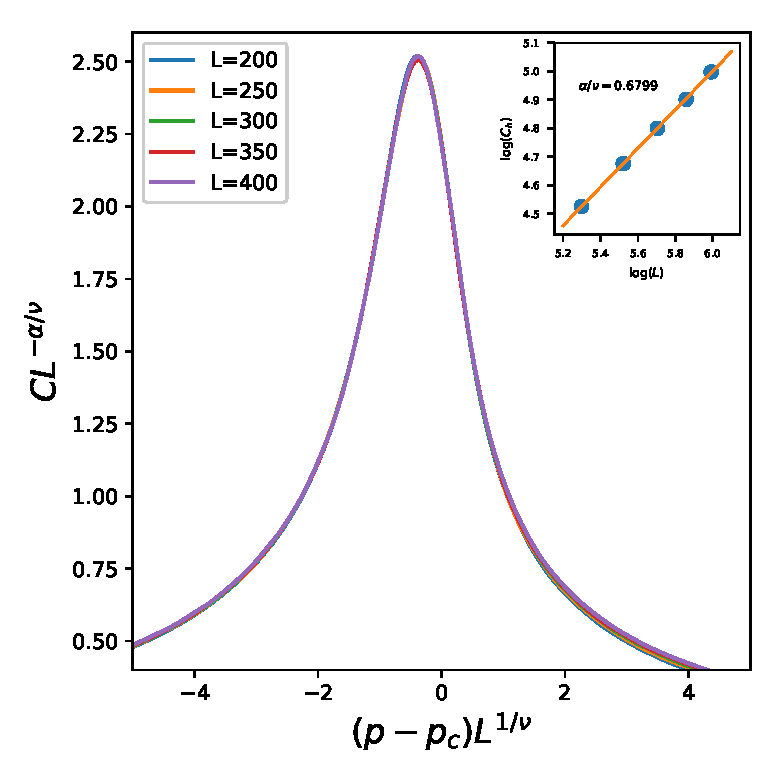
\includegraphics[width=\linewidth]{{{L0/sq_lattice_site_percolation_periodic__specific_heat-data_collapse-pc0.5927_alpha_0.6799_nu_0.750}}}
				\caption{L0}
			\end{subfigure}
			\begin{subfigure}{0.329\textwidth}
				\centering
				\includegraphics[width=\linewidth]{{{sq_lattice_site_percolation_ballistic_deposition_L1_periodic__specific_heat-data_collapse-pc0.5782_alpha_0.6712_nu_0.736-with}}}
				\caption{L1}
			\end{subfigure}
			\begin{subfigure}{0.329\textwidth}
				\centering
				\includegraphics[width=\linewidth]{{{sq_lattice_site_percolation_ballistic_deposition_L2_periodic__specific_heat-data_collapse-pc0.5701_alpha_0.6712_nu_0.721-with}}}
				\caption{L2}
			\end{subfigure}
			\caption{$C L^{-\alpha/\nu}$ vs $(p-p_c) L^{1/\nu}$}
			\label{fig:specific-heat-data-collapse-graph}
		\end{figure}
	\subsection{Order Parameter and finding $\beta$}
	\label{subsect:order-parameter}
		Order parameter, also knows as the percolation strength, is ,along with entropy, an important quantity in the study of phase transition. It is denoted as $P(p,L)$. Using the definition \ref{def:order-parameter-2} we obtain the order parameter for our system and it is shown in the figure \ref{fig:order-parameter}. Since using spanning cluster and the largest cluster gives the same exponent, it really does not matter which one we use. But in our case there is a boundary of the system, which we define as periodic. Hence using spanning cluster is appropriate.
		\begin{figure}
			\begin{subfigure}{0.329\textwidth}
				\centering
				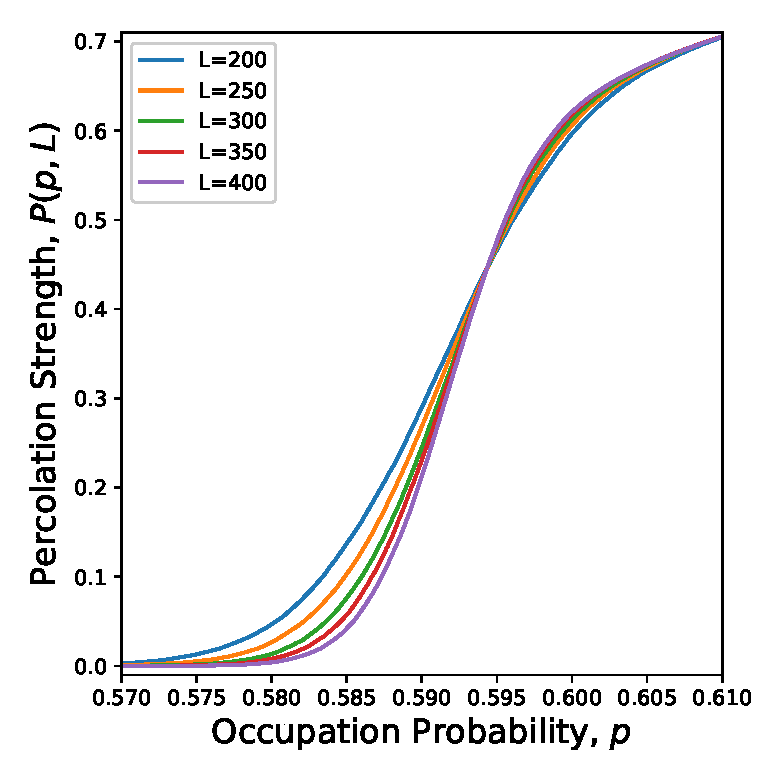
\includegraphics[width=\linewidth]{{{L0/sq_lattice_site_percolation_periodic_-spanning-_order_parameter-pc0.5927}}}
				\caption{L0}
			\end{subfigure}
			\begin{subfigure}{0.329\textwidth}
				\centering
				\includegraphics[width=\linewidth]{{{sq_lattice_site_percolation_ballistic_deposition_L1_periodic_-spanning-_order_parameter-pc0.5782}}}
				\caption{L1}
			\end{subfigure}
			\begin{subfigure}{0.329\textwidth}
				\centering
				\includegraphics[width=\linewidth]{{{sq_lattice_site_percolation_ballistic_deposition_L2_periodic_-spanning-_order_parameter-pc0.5701}}}
				\caption{L2}
			\end{subfigure}
			\caption{Order Parameter, $P(p,L)$ vs Occupation Probability, $p$}
			\label{fig:order-parameter}
		\end{figure}
		Using the exponent $1/\nu$ obtained in section \ref{subsect:spanning-probability-and-one-by-nu} we scale the $x$-values as $(p-p_c)L^{1/\nu}$ and get the following figure \ref{fig:order-parameter-x-scaled}.
		\begin{figure}
			\begin{subfigure}{0.329\textwidth}
				\centering
				\includegraphics[width=\linewidth]{{{sq_lattice_site_percolation_periodic_-spanning-_order_parameter-x-scaled-pc0.5927}}}
				\caption{L0}
			\end{subfigure}
			\begin{subfigure}{0.329\textwidth}
				\centering
				\includegraphics[width=\linewidth]{{{sq_lattice_site_percolation_ballistic_deposition_L1_periodic_-spanning-_order_parameter-x-scaled-pc0.5782}}}
				\caption{L1}
			\end{subfigure}
			\begin{subfigure}{0.329\textwidth}
				\centering
				\includegraphics[width=\linewidth]{{{sq_lattice_site_percolation_ballistic_deposition_L2_periodic_-spanning-_order_parameter-x-scaled-pc0.5701}}}
				\caption{L2}
			\end{subfigure}
			\caption{Order Parameter, $P(p,L)$ vs Occupation Probability, $p$}
			\label{fig:order-parameter-x-scaled}
			\caption{$P(p,L)$ vs $(p-p_c) L ^{1/\nu}$}
		\end{figure}
 	    Then in figure \ref{fig:order-parameter-x-scaled} we draw a vertical line where there are several horizontal lines. We measure the height of the lines and call it $P_h$ and after plotting $\log(P_h)$ vs $\log(L)$ (inset of figure \ref{fig:order-parameter-data-collapse})we get the exponent $\beta/\nu$ from it's slope and obtain exponent $\beta$ by dividing $\beta/\nu$ by $1/\nu$.
 	    Using the FSS hypothesis \ref{subsect:FSS} we plot $PL^{\beta/\nu}$ versus $(p-p_c)L^1/\nu$ and get a good data collapse which is shown in figure \ref{fig:order-parameter-data-collapse}.
		\begin{figure}
			\begin{subfigure}{0.329\textwidth}
				\centering
				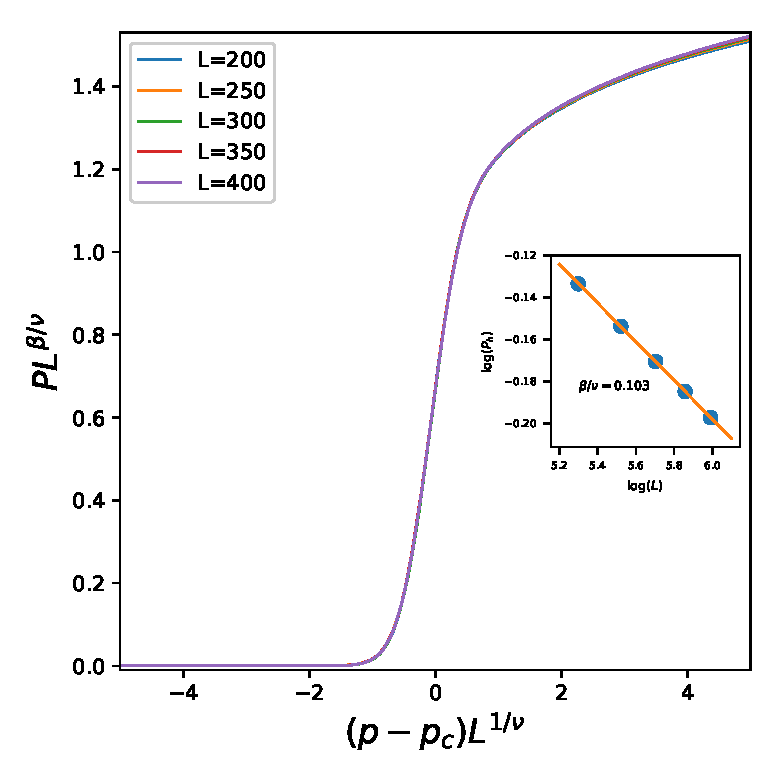
\includegraphics[width=\linewidth]{{{L0/sq_lattice_site_percolation_periodic_-spanning-_order_parameter-data_collapse-pc0.5927_beta_0.103_nu_0.750}}}
				\caption{L0}
			\end{subfigure}
			\begin{subfigure}{0.329\textwidth}
				\centering
				\includegraphics[width=\linewidth]{{{sq_lattice_site_percolation_ballistic_deposition_L1_periodic_-spanning-_order_parameter-data_collapse-pc0.5782_beta_0.103_nu_0.736}}}
				\caption{L1}
			\end{subfigure}
			\begin{subfigure}{0.329\textwidth}
				\centering
				\includegraphics[width=\linewidth]{{{sq_lattice_site_percolation_ballistic_deposition_L2_periodic_-spanning-_order_parameter-data_collapse-pc0.5701_beta_0.098_nu_0.721}}}
				\caption{L2}
			\end{subfigure}
			\caption{$P L^{\beta/\nu}$ vs $(p-p_c) L ^{1/\nu}$}
			\label{fig:order-parameter-data-collapse}
		\end{figure}
	\subsection{Susceptibility and finding $\gamma$}
	Susceptibility is defined as the derivative of the order parameter $P(p,L)$ with respect to the control parameter $p$,i.e., $\chi = \frac{dP}{dp}$. Using this definition we obtain the graph of susceptibility \ref{fig:susceptibility}. And if we scale the $x$ values and plot $\chi$ vs $(p-p_c)L^{1/\nu}$ we get all the peak point aligned (figure \ref{fig:susceptibility-x-scaled}). Note that the value of $1/\nu$ is known from section \ref{subsect:spanning-probability-and-one-by-nu}. Then we take the reading of the height of each line and call it $\chi_h$. Since each line represents a different lattice size, plotting $\log(\chi_h)$ vs $\log(L)$ gives the slope $\gamma/\nu$. And using the FSS hypothesis we plot $\chi L^{-\gamma/\nu}$ vs $(p-p_c)L^{1/\nu}$ and obtain a perfect data collapse. It is shown in figure \ref{fig:susceptibility-data-collapse}. We obtain the values of $\gamma$ to be $0.8543,0.8542,0.882$.
		\begin{figure}
			\begin{subfigure}{0.329\textwidth}
				\centering
				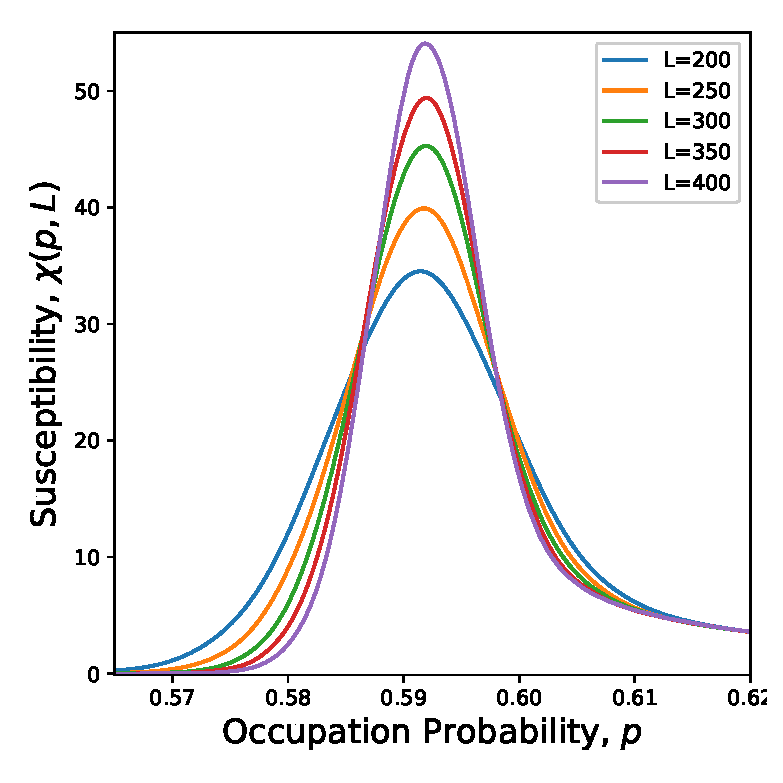
\includegraphics[width=\linewidth]{{{L0/sq_lattice_site_percolation_periodic__susceptibility-pc0.5927}}}
				\caption{L0}
			\end{subfigure}
			\begin{subfigure}{0.329\textwidth}
				\centering
				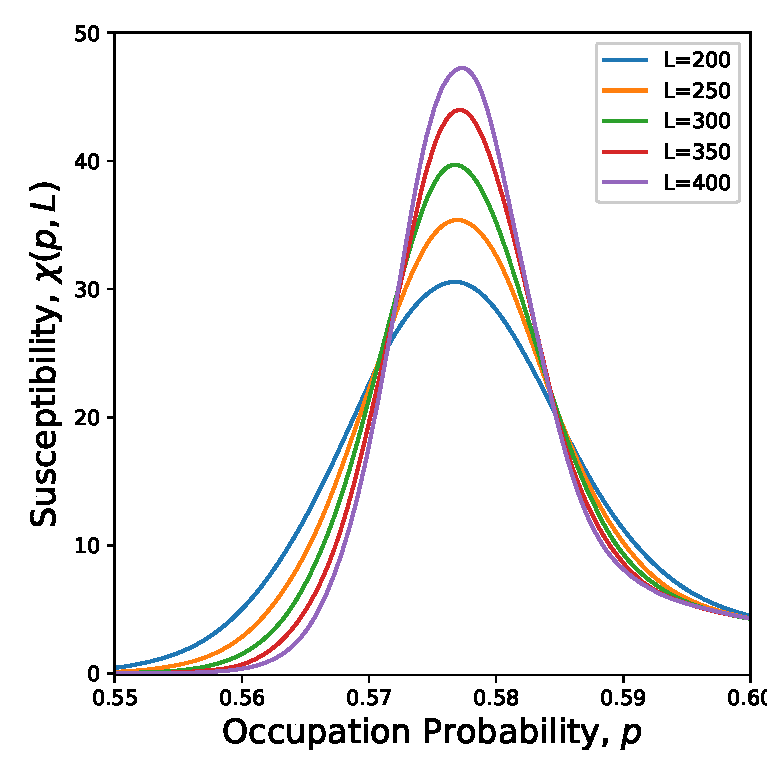
\includegraphics[width=\linewidth]{{{L1/sq_lattice_site_percolation_ballistic_deposition_L1_periodic__susceptibility-pc0.5782}}}
				\caption{L1}
			\end{subfigure}
			\begin{subfigure}{0.329\textwidth}
				\centering
				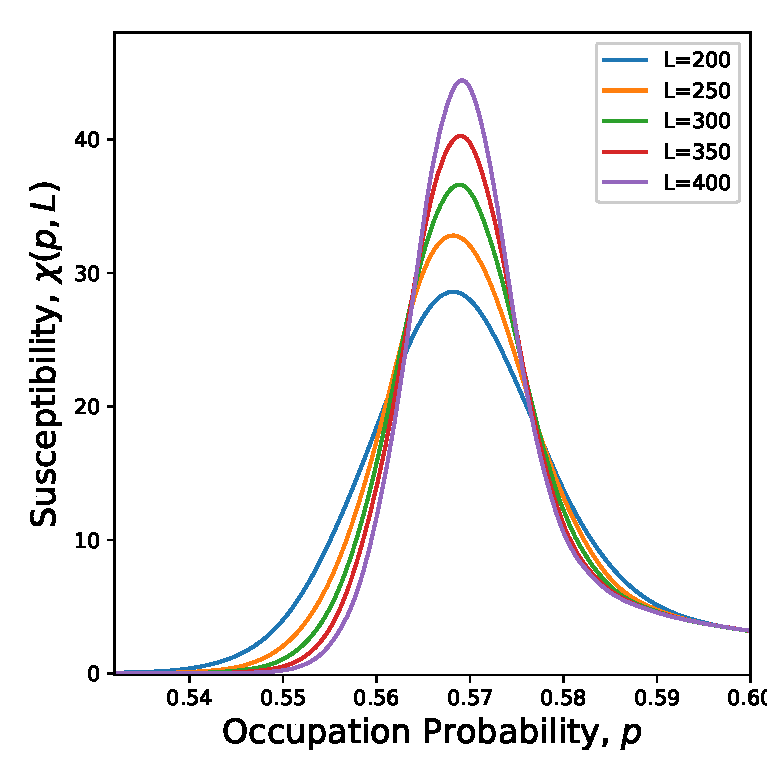
\includegraphics[width=\linewidth]{{{L2/sq_lattice_site_percolation_ballistic_deposition_L2_periodic__susceptibility-pc0.5701}}}
				\caption{L2}
			\end{subfigure}
			\caption{Susceptibility, $\chi(p,L)$ vs Occupation Probability, $p$}
			\label{fig:susceptibility}
		\end{figure}
		\begin{figure}
				\begin{subfigure}{0.329\textwidth}
				\centering
				\includegraphics[width=\linewidth]{{{sq_lattice_site_percolation_periodic__susceptibility-x-scaled-pc0.5927_gamma_0.6407_nu_0.750}}}
				\caption{L0}
			\end{subfigure}
			\begin{subfigure}{0.329\textwidth}
				\centering
				\includegraphics[width=\linewidth]{{{sq_lattice_site_percolation_ballistic_deposition_L1_periodic__susceptibility-x-scaled-pc0.5782_gamma_0.6287_nu_0.736}}}
				\caption{L1}
			\end{subfigure}
			\begin{subfigure}{0.329\textwidth}
				\centering
				\includegraphics[width=\linewidth]{{{sq_lattice_site_percolation_ballistic_deposition_L2_periodic__susceptibility-x-scaled-pc0.5701_gamma_0.6362_nu_0.721}}}
				\caption{L2}
			\end{subfigure}
			\caption{$\chi(p,L)$ vs $(p-p_c) L ^{1/\nu}$}
			\label{fig:susceptibility-x-scaled}
		\end{figure}
		\begin{figure}
			\begin{subfigure}{0.329\textwidth}
				\centering
				\includegraphics[width=\linewidth]{{{sq_lattice_site_percolation_periodic__susceptibility-data_collapse-pc0.5927_gamma_0.6407_nu_0.750}}}
				\caption{L0}
			\end{subfigure}
			\begin{subfigure}{0.329\textwidth}
				\centering
				\includegraphics[width=\linewidth]{{{sq_lattice_site_percolation_ballistic_deposition_L1_periodic__susceptibility-data_collapse-pc0.5782_gamma_0.6287_nu_0.736}}}
				\caption{L1}
			\end{subfigure}
			\begin{subfigure}{0.329\textwidth}
				\centering
				\includegraphics[width=\linewidth]{{{sq_lattice_site_percolation_ballistic_deposition_L2_periodic__susceptibility-data_collapse-pc0.5701_gamma_0.6362_nu_0.721}}}
				\caption{L2}
			\end{subfigure}
			\caption{$\chi L^{\gamma/\nu}$ vs $(p-p_c) L ^{1/\nu}$}
			\label{fig:susceptibility-data-collapse}
		\end{figure}
	
	
	
	\subsection{Cluster Size Distribution}
		Cluster size $S$ is related to $n_S$ by the relation
		\begin{equation}
			n_S \sim S^{-\tau}
		\end{equation}
		taking log on both sides gives us
		\begin{equation}
			\log n_S = -\tau \log S
		\end{equation}
		Thus the exponent $\tau$ gives us the information of the average cluster size. At the critical point all the cluster (apart from the largest ones and smallest ones) follows a pattern. Their size is related to the number times of they appear.
		\begin{figure}
			\caption{Number of cluster of size $s$, $n_s$ vs size of the cluster $s$}
		\end{figure}
		\begin{figure}
			\begin{subfigure}{0.329\textwidth}
			\centering
			\includegraphics[width=\linewidth]{{{sq_lattice_site_percolation_periodic_cluster-size-distribution_cluster_by_bond}}}
			\caption{L0}
			\end{subfigure}
			\begin{subfigure}{0.329\textwidth}
			\centering
			\includegraphics[width=\linewidth]{{{sq_lattice_site_percolation_ballistic_deposition_L1_periodic__cluster_by_bond_cluster-size-distribution-log-log_cluster_by_bond}}}
			\caption{L1}
			\end{subfigure}
			\begin{subfigure}{0.329\textwidth}
			\centering
			\includegraphics[width=\linewidth]{{{sq_lattice_site_percolation_ballistic_deposition_L2_periodic__cluster_by_bond_cluster-size-distribution-log-log_cluster_by_bond}}}
			\caption{L2}
			\end{subfigure}
			\caption{$\log(n_s)$ vs $\log(s)$}
		\end{figure}
	$n_s$ vs $s$ graph



	\subsection{Order-Disorder Transition}
	    Phase transition is an order-disorder transition. There is a critical point which separates the two regions. Before the critical point the system is in disordered phase and after it is in ordered phase when we increase temperature in thermodynamics. Behavior of two phases are completely different. It's astonishing how the behavior changes. In percolation theory, this order disorder transition is different than in thermodynamics. Here disordered means uncertainty, since we are dealing with a system where probability is the control parameter (the occupation probability $p$). When $p$ is minimum all clusters are disconnected and have size of unity. This means that we can to pick a cluster with probability $\frac{1}{2L^2}$, where $L$ is the lattice size and $2L^2$ is the number of bonds in the lattice. That's why entropy is maximum and order parameter is minimum in this region. Now as we keep occupying the lattice clusters of different size arises, and at some point a miracle happens. It is the critical point where the transition occurs. A cluster appears for the first time which spans the entire lattice either horizontally or vertically. And in case of periodic condition the cluster wraps the lattice all the way around it. This cluster is called the spanning (wrapping) cluster in non-periodic (periodic) condition. The probability of picking this cluster at random is always larger than picking any other clusters. Thus system goes to the ordered state. And if we keep occupying the lattice at some point all cluster are joined to form one cluster. Thus picking this cluster at random has no uncertainty, meaning we have reached the entirely ordered phase. Here entropy is minimum and ordered parameter is maximum. A graph \ref{fig:ordered-disordered-transition} containing both entropy and order parameter can show this process. We have normalized the entropy (figure \ref{fig:entropy}) to match with the order parameter (figure \ref{fig:order-parameter}).

		\begin{figure}
			\begin{subfigure}{0.329\textwidth}
				\centering
				\includegraphics[width=\linewidth]{{{sq_lattice_site_percolation_periodic__entropy_by_site-entropy-order_parameter-L400}}}
				\caption{L0}
			\end{subfigure}
			\begin{subfigure}{0.329\textwidth}
				\centering
				\includegraphics[width=\linewidth]{{{sq_lattice_site_percolation_ballistic_deposition_L1_periodic_-entropy-order_parameter-L400}}}
				\caption{L1}
			\end{subfigure}
			\begin{subfigure}{0.329\textwidth}
				\centering
				\includegraphics[width=\linewidth]{{{sq_lattice_site_percolation_ballistic_deposition_L2_periodic_-entropy-order_parameter-L400}}}
				\caption{L2}
			\end{subfigure}
			\caption{$H(p,L)/H(0,L)$ or $P(p,L)/P(1,L)$ vs $p$}
			\label{fig:ordered-disordered-transition}
		\end{figure}
	\subsection{Fractal Dimension}
		At critical point the square lattice shows the property of a fractal. A fractal is an object which occupies less space than it is embedded. For example a piece of cheese is a 3D fractal, since there are holes in the cheese which is empty. We use the relation
		\begin{equation}
			S \sim L^{d_f}
			\label{eqn:fractal-dim}
		\end{equation}
		taking $\log$ we get
		\begin{equation}
			\log(S) = d_f \log(L)
		\end{equation}
		Here $S$ is the average size of the spanning cluster at critical point. Using this we get the figure \ref{fig:fractal-dimension}. And we obtain fractal dimension $d_f$ for $L0,L1,L2$ which is listed in \ref{tab:exponents}. 
		\begin{figure}
			\begin{subfigure}{0.329\textwidth}
				\centering
				\includegraphics[width=\linewidth]{{{sq_lattice_site_percolation_periodic_-fractal_dimension_1.89394}}}
				\caption{L0}
			\end{subfigure}
			\begin{subfigure}{0.329\textwidth}
				\centering
				\includegraphics[width=\linewidth]{{{sq_lattice_site_percolation_ballistic_deposition_L1_periodic_-fractal_dimension_1.8995}}}
				\caption{L1}
			\end{subfigure}
			\begin{subfigure}{0.329\textwidth}
				\centering
				\includegraphics[width=\linewidth]{{{sq_lattice_site_percolation_ballistic_deposition_L2_periodic_-fractal_dimension_1.9081}}}
				\caption{L2}
			\end{subfigure}
			\label{fig:fractal-dimension}
			\caption{$\log(S)$ vs $\log(L)$}
		\end{figure}
		Fractal dimension gives us the information about the size of the spanning(wrapping) cluster. If the lattice size is known we can estimate the average size of the spanning cluster using $d_f$ and \ref{eqn:fractal-dim}.
